\subsection{Gtransfo\-Quad  Class Reference}
\label{class_gtransfoquad}\index{GtransfoQuad@{Gtransfo\-Quad}}
implements the quadratic transformations (12 real coefficients). 


{\tt \#include $<$gtransfo.h$>$}

Inheritance diagram for Gtransfo\-Quad::\begin{figure}[H]
\begin{center}
\leavevmode
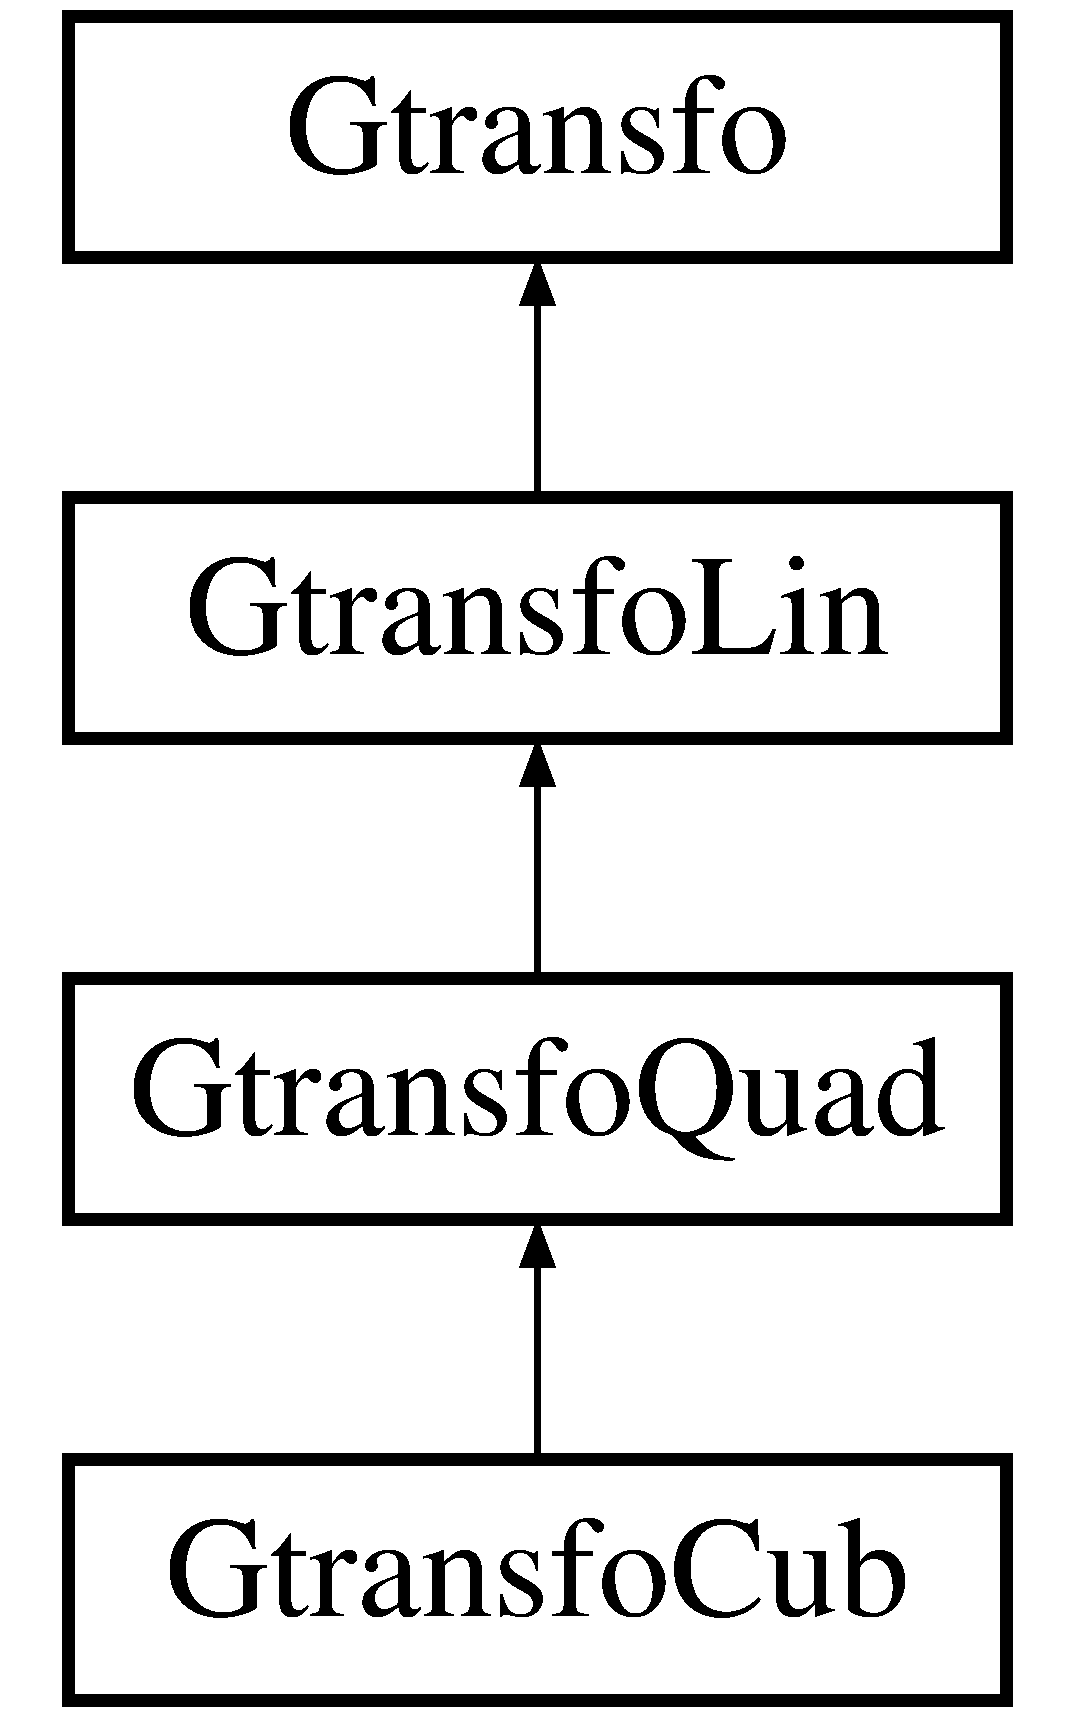
\includegraphics[height=4cm]{class_gtransfoquad}
\end{center}
\end{figure}
\subsubsection*{Public Methods}
\begin{CompactItemize}
\item 
\index{GtransfoQuad@{GtransfoQuad}!GtransfoQuad@{Gtransfo\-Quad}}\index{GtransfoQuad@{GtransfoQuad}!GtransfoQuad@{Gtransfo\-Quad}}
{\bf Gtransfo\-Quad} ()\label{class_gtransfoquad_a0}

\begin{CompactList}\small\item\em the default constructor constructs the do-nothing transformation.\item\end{CompactList}\item 
\index{GtransfoQuad@{GtransfoQuad}!GtransfoQuad@{Gtransfo\-Quad}}\index{GtransfoQuad@{GtransfoQuad}!GtransfoQuad@{Gtransfo\-Quad}}
{\bf Gtransfo\-Quad} (const {\bf Gtransfo\-Lin} \&Lin)\label{class_gtransfoquad_a1}

\begin{CompactList}\small\item\em upgrade a linear transfo to a Quad one.\item\end{CompactList}\item 
\index{operator *@{operator $\ast$}!GtransfoQuad@{Gtransfo\-Quad}}\index{GtransfoQuad@{GtransfoQuad}!operator *@{operator $\ast$}}
Gtransfo\-Quad {\bf operator $\ast$} (const {\bf Gtransfo\-Lin} \&R) const\label{class_gtransfoquad_a2}

\begin{CompactList}\small\item\em enables to combine linear tranformations: T1=T2$\ast$T3 is legal.\item\end{CompactList}\item 
\index{apply@{apply}!GtransfoQuad@{Gtransfo\-Quad}}\index{GtransfoQuad@{GtransfoQuad}!apply@{apply}}
void {\bf apply} (const double Xin, const double Yin, double \&Xout, double \&Yout) const\label{class_gtransfoquad_a3}

\item 
\index{dump@{dump}!GtransfoQuad@{Gtransfo\-Quad}}\index{GtransfoQuad@{GtransfoQuad}!dump@{dump}}
void {\bf dump} (ostream \&stream=cout) const\label{class_gtransfoquad_a4}

\begin{CompactList}\small\item\em dumps the transfo coefficients to stream.\item\end{CompactList}\item 
double {\bf fit} (const Star\-Match\-List \&List, const {\bf Gtransfo} $\ast$Prior\-Transfo=NULL, const {\bf Gtransfo} $\ast$Posterior\-Transfo=NULL)
\begin{CompactList}\small\item\em fits a transfo to a list of star pairs (p1,p2).\item\end{CompactList}\item 
\index{Clone@{Clone}!GtransfoQuad@{Gtransfo\-Quad}}\index{GtransfoQuad@{GtransfoQuad}!Clone@{Clone}}
{\bf Gtransfo}$\ast$ {\bf Clone} () const\label{class_gtransfoquad_a6}

\begin{CompactList}\small\item\em returns a copy (allocated by new) of the transformation.\item\end{CompactList}\item 
\index{ReduceCompo@{ReduceCompo}!GtransfoQuad@{Gtransfo\-Quad}}\index{GtransfoQuad@{GtransfoQuad}!ReduceCompo@{Reduce\-Compo}}
{\bf Gtransfo}$\ast$ {\bf Reduce\-Compo} (const {\bf Gtransfo} $\ast$Right) const\label{class_gtransfoquad_a7}

\begin{CompactList}\small\item\em allow composition of transformations regardless of their actual types.see {\bf Gtransfo\-Compose}() {\rm (p.\,\pageref{gtransfo_h_a1})} for a user callable entry.\item\end{CompactList}\item 
{\bf Gtransfo}$\ast$ {\bf Inverse\-Transfo} (const double Precision, const {\bf Frame} \&Region) const
\begin{CompactList}\small\item\em returns an inverse transfo.\item\end{CompactList}\item 
void {\bf Derivative} (const {\bf Point} \&Where, {\bf Gtransfo\-Lin} \&Derivative, const double Step=0.01) const
\begin{CompactList}\small\item\em Computes the local Derivative of a transfo. Step is used for numerical derivation.\item\end{CompactList}\item 
\index{LinearApproximation@{LinearApproximation}!GtransfoQuad@{Gtransfo\-Quad}}\index{GtransfoQuad@{GtransfoQuad}!LinearApproximation@{Linear\-Approximation}}
{\bf Gtransfo\-Lin} {\bf Linear\-Approximation} (const {\bf Point} \&Where, const double step=0.01) const\label{class_gtransfoquad_a10}

\begin{CompactList}\small\item\em linear (local) approximation.\item\end{CompactList}\item 
\index{A1X2@{A1X2}!GtransfoQuad@{Gtransfo\-Quad}}\index{GtransfoQuad@{GtransfoQuad}!A1X2@{A1X2}}
double {\bf A1X2} () const\label{class_gtransfoquad_a11}

\item 
\index{A1XY@{A1XY}!GtransfoQuad@{Gtransfo\-Quad}}\index{GtransfoQuad@{GtransfoQuad}!A1XY@{A1XY}}
double {\bf A1XY} () const\label{class_gtransfoquad_a12}

\item 
\index{A1Y2@{A1Y2}!GtransfoQuad@{Gtransfo\-Quad}}\index{GtransfoQuad@{GtransfoQuad}!A1Y2@{A1Y2}}
double {\bf A1Y2} () const\label{class_gtransfoquad_a13}

\item 
\index{A2X2@{A2X2}!GtransfoQuad@{Gtransfo\-Quad}}\index{GtransfoQuad@{GtransfoQuad}!A2X2@{A2X2}}
double {\bf A2X2} () const\label{class_gtransfoquad_a14}

\item 
\index{A2XY@{A2XY}!GtransfoQuad@{Gtransfo\-Quad}}\index{GtransfoQuad@{GtransfoQuad}!A2XY@{A2XY}}
double {\bf A2XY} () const\label{class_gtransfoquad_a15}

\item 
\index{A2Y2@{A2Y2}!GtransfoQuad@{Gtransfo\-Quad}}\index{GtransfoQuad@{GtransfoQuad}!A2Y2@{A2Y2}}
double {\bf A2Y2} () const\label{class_gtransfoquad_a16}

\item 
\index{Npar@{Npar}!GtransfoQuad@{Gtransfo\-Quad}}\index{GtransfoQuad@{GtransfoQuad}!Npar@{Npar}}
int {\bf Npar} () const\label{class_gtransfoquad_a17}

\begin{CompactList}\small\item\em returns the number of parameters (to compute chi2's).\item\end{CompactList}\item 
\index{Degree@{Degree}!GtransfoQuad@{Gtransfo\-Quad}}\index{GtransfoQuad@{GtransfoQuad}!Degree@{Degree}}
virtual int {\bf Degree} () const\label{class_gtransfoquad_a18}

\item 
\index{GtransfoQuad@{GtransfoQuad}!GtransfoQuad@{Gtransfo\-Quad}}\index{GtransfoQuad@{GtransfoQuad}!GtransfoQuad@{Gtransfo\-Quad}}
{\bf Gtransfo\-Quad} (double ox, double oy, double aa11, double aa12, double aa21, double aa22, double aa1x2, double aa1xy, double aa1y2, double aa2x2, double aa2xy, double aa2y2)\label{class_gtransfoquad_a19}

\end{CompactItemize}
\subsubsection*{Protected Methods}
\begin{CompactItemize}
\item 
\index{identity@{identity}!GtransfoQuad@{Gtransfo\-Quad}}\index{GtransfoQuad@{GtransfoQuad}!identity@{identity}}
void {\bf identity} ()\label{class_gtransfoquad_b0}

\end{CompactItemize}
\subsubsection*{Protected Attributes}
\begin{CompactItemize}
\item 
\index{a1x2@{a1x2}!GtransfoQuad@{Gtransfo\-Quad}}\index{GtransfoQuad@{GtransfoQuad}!a1x2@{a1x2}}
double {\bf a1x2}\label{class_gtransfoquad_n0}

\item 
\index{a1xy@{a1xy}!GtransfoQuad@{Gtransfo\-Quad}}\index{GtransfoQuad@{GtransfoQuad}!a1xy@{a1xy}}
double {\bf a1xy}\label{class_gtransfoquad_n1}

\item 
\index{a1y2@{a1y2}!GtransfoQuad@{Gtransfo\-Quad}}\index{GtransfoQuad@{GtransfoQuad}!a1y2@{a1y2}}
double {\bf a1y2}\label{class_gtransfoquad_n2}

\item 
\index{a2x2@{a2x2}!GtransfoQuad@{Gtransfo\-Quad}}\index{GtransfoQuad@{GtransfoQuad}!a2x2@{a2x2}}
double {\bf a2x2}\label{class_gtransfoquad_n3}

\item 
\index{a2xy@{a2xy}!GtransfoQuad@{Gtransfo\-Quad}}\index{GtransfoQuad@{GtransfoQuad}!a2xy@{a2xy}}
double {\bf a2xy}\label{class_gtransfoquad_n4}

\item 
\index{a2y2@{a2y2}!GtransfoQuad@{Gtransfo\-Quad}}\index{GtransfoQuad@{GtransfoQuad}!a2y2@{a2y2}}
double {\bf a2y2}\label{class_gtransfoquad_n5}

\end{CompactItemize}
\subsubsection*{Friends}
\begin{CompactItemize}
\item 
class {\bf operator $\ast$}
\end{CompactItemize}


\subsubsection{Detailed Description}
implements the quadratic transformations (12 real coefficients).



\subsubsection{Member Function Documentation}
\index{GtransfoQuad@{Gtransfo\-Quad}!Derivative@{Derivative}}
\index{Derivative@{Derivative}!GtransfoQuad@{Gtransfo\-Quad}}
\paragraph{\setlength{\rightskip}{0pt plus 5cm}void Gtransfo\-Quad::Derivative (const {\bf Point} \& {\em Where}, {\bf Gtransfo\-Lin} \& {\em Derivative}, const double {\em Step} = 0.01) const\hspace{0.3cm}{\tt  [virtual]}}\hfill\label{class_gtransfoquad_a9}


Computes the local Derivative of a transfo. Step is used for numerical derivation.

the Derivative is represented by a {\bf Gtransfo\-Lin} {\rm (p.\,\pageref{class_gtransfolin})}, in which (hopefully), the offset terms are zero. Derivative should  transform a vector of offsets into a vector of offsets. 

Reimplemented from {\bf Gtransfo\-Lin} {\rm (p.\,\pageref{class_gtransfolin_a5})}.\index{GtransfoQuad@{Gtransfo\-Quad}!InverseTransfo@{InverseTransfo}}
\index{InverseTransfo@{InverseTransfo}!GtransfoQuad@{Gtransfo\-Quad}}
\paragraph{\setlength{\rightskip}{0pt plus 5cm}{\bf Gtransfo}$\ast$ Gtransfo\-Quad::Inverse\-Transfo (const double {\em Precision}, const {\bf Frame} \& {\em Region}) const\hspace{0.3cm}{\tt  [virtual]}}\hfill\label{class_gtransfoquad_a8}


returns an inverse transfo.

Precision and Region refer to the \char`\"{}input\char`\"{} side of this,  and hence to the output side of the returned {\bf Gtransfo} {\rm (p.\,\pageref{class_gtransfo})}. 

Reimplemented from {\bf Gtransfo\-Lin} {\rm (p.\,\pageref{class_gtransfolin_a14})}.\index{GtransfoQuad@{Gtransfo\-Quad}!fit@{fit}}
\index{fit@{fit}!GtransfoQuad@{Gtransfo\-Quad}}
\paragraph{\setlength{\rightskip}{0pt plus 5cm}double Gtransfo\-Quad::fit (const Star\-Match\-List \& {\em List}, const {\bf Gtransfo} $\ast$ {\em Prior\-Transfo} = NULL, const {\bf Gtransfo} $\ast$ {\em Posterior\-Transfo} = NULL)\hspace{0.3cm}{\tt  [virtual]}}\hfill\label{class_gtransfoquad_a5}


fits a transfo to a list of star pairs (p1,p2).

After the fit this(Prior\-Transfo(p1)) yields approximately Posterior\-Transfo(p2). The returned value is the chi2. 

Reimplemented from {\bf Gtransfo\-Lin} {\rm (p.\,\pageref{class_gtransfolin_a9})}.

Reimplemented in {\bf Gtransfo\-Cub} {\rm (p.\,\pageref{class_gtransfocub_a6})}.

The documentation for this class was generated from the following file:\begin{CompactItemize}
\item 
{\bf gtransfo.h}\end{CompactItemize}
